\documentclass[11pt,a4paper]{article}
\usepackage[utf8]{inputenc}
\usepackage[hmargin=2.0cm,vmargin=2.5cm,bindingoffset=0.5cm]{geometry}
\usepackage{amsfonts}
\usepackage{amsmath,amsthm,amssymb}
\allowdisplaybreaks
\usepackage{hyperref}
\usepackage{graphicx}
\usepackage{tikz}
\usepackage{mathtools}
\DeclarePairedDelimiter\ceil{\lceil}{\rceil}
\DeclarePairedDelimiter\floor{\lfloor}{\rfloor}
%\usepackage{float}
\usepackage{placeins}
\usepackage{diagbox}
\DeclareMathOperator{\Tr}{Tr}
\newtheorem{thm}{Theorem}
\usepackage{subcaption}
%\usepackage{subfigure}
\usepackage[english]{babel}
\author{Mohit}
\title{Counter-diabatic driving using Floquet engineering}
\begin{document}
\maketitle
%\tableofcontents

\section{CD driving}
 \begin{equation}
 H_0= - J \sum_j (c^{\dagger}_{j+1} c_j+ \mbox{h.c}) + \sum_j V_j (\lambda) c^{\dagger}_{j} c_j
 \end{equation}
For this problem, approximate gauge potential is chosen to be $A_{\lambda}^*= i \sum_j \alpha_j (c^{\dagger}_{j+1} c_j- h.c)$.

On minimizing action, we get 
\begin{align*}
-3 J^2 (\alpha_{j+1}+ \alpha_{j-1})+ (6 J^2 + (V_{j+1}- V_{j})^2) \alpha_j= - J \partial_{\lambda} (V_{j+1}- V_{j}) \\
\end{align*}


\begin{figure}[!ht]
\begin{center}
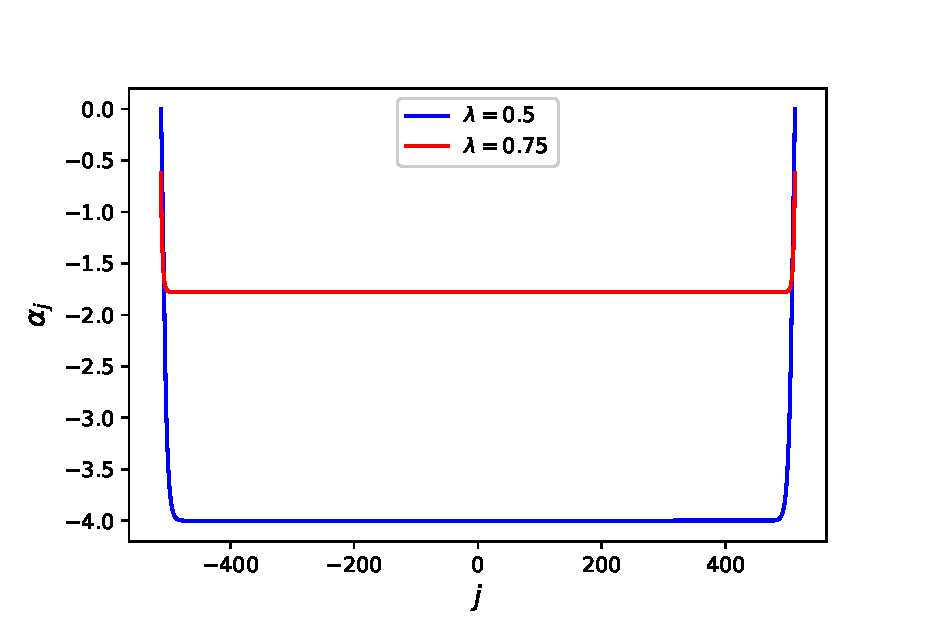
\includegraphics[scale=0.5]{pics/alpha_j_linear_potn.eps}
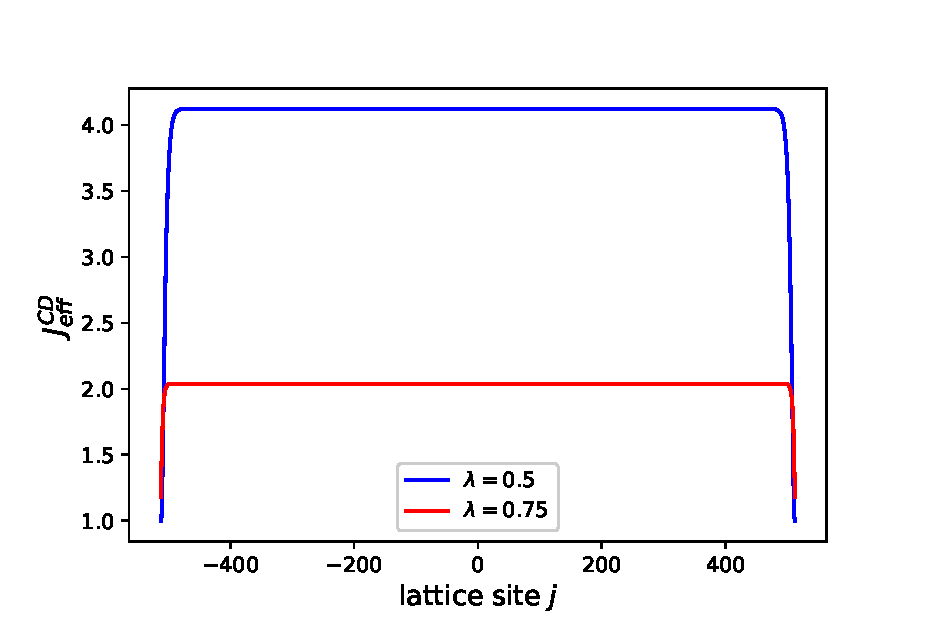
\includegraphics[scale=0.5]{pics/j_eff_cd.eps}\\
\caption{a) $\alpha_j$ for linear potential with vanishing boundary condition b) Effective hopping strength}
\end{center}
\end{figure}

\begin{align*}
H_{CD}&= H_0 + \dot{\lambda} A_{\lambda}=  \sum_j J^{CD}_j (c^{\dagger}_{i+1} c_i+ h.c) + \sum_j U_j  c^{\dagger}_{i} c_i
\end{align*}

where 
\begin{align*}
J^{CD}_j= J \sqrt{1 + (\dot{\lambda} \alpha_j/J)^2} \quad U_j = V_j( \lambda) - \sum_i^j \dfrac{J}{J^2 + (\dot{\lambda} \alpha_i/J)^2} (\ddot{\lambda} \alpha_j + \dot{\lambda}^2 \partial_{\lambda} \alpha_j)
\end{align*}

Over here, I am going to work with $\dot{\lambda}=1$ and $L=1024$.
\section{Floquet driving}

\begin{align*}
H = H_0 + H_1 = J\sum_j (c_{j+1}^{\dagger} c_j  + \mbox{h.c}) + \cos(\omega t) \sum_j A_j  c_j^{\dagger} c_j
\end{align*}
We would go to the rotating frame $|\psi_{rot} \rangle= V^{\dagger}|\psi_{lab} \rangle$
where $V=\exp(-i \sin(\omega t)/ \omega \sum_j A_j  c_j^{\dagger} c_j)$.

\begin{align*}
H_{rot}&= V^{\dagger} H V- i V^{\dagger} \dot{V}\\
&=V^{\dagger} H_0 V + \cos(\omega t) \sum_j A_j  c_j^{\dagger} c_j + i^2 \cos(\omega t) \sum_j A_j  c_j^{\dagger} c_j \\
&=V^{\dagger} H_0 V =V^{\dagger} c_{j+1}^{\dagger}V V^{\dagger} c_j V  + \mbox{h.c}
\end{align*}

Using $[n_j,c_j ]= -c_j$ and $[n_j,c_j^{\dagger} ]= c_j^{\dagger}$

\begin{align*}
H_{rot}&= J\sum_j   ( g^{j, j+1} c_{j+1}^{\dagger} c_j + \mbox{h.c}) \quad \mbox{where } ~ g^{j, j+1}= \exp\left(i \sin(\omega t) \dfrac{A_{j+1}- A_j}{\omega}\right)
\end{align*}




\begin{align*}
H_F^{(0)}&= \dfrac{1}{T}   \sum_j \int_{t_0}^{T+t_0}(c_{j+1}^{\dagger} c_j \exp\left(i \sin(\omega t) \dfrac{A_{j+1}- A_j}{\omega}\right) dt + \mbox{h.c})\\
&= \sum_j J_{j}^F (c_{j+1}^{\dagger} c_j + \mbox{h.c}) \quad \mbox{where} ~ J_{j}^F=J^F \mathcal{J}_0 \left(\dfrac{A_{j+1}- A_j}{\omega}\right)
\end{align*}


%A necessary condition for cold atom experiments to work is that the driving frequency be smaller than the band gap between the lowest two Bloch bands, or otherwise higher bands will get populated.


\section{Linear potential}
We choose $V(j, \lambda)= j \lambda$.



\begin{figure}[!ht]
\begin{center}
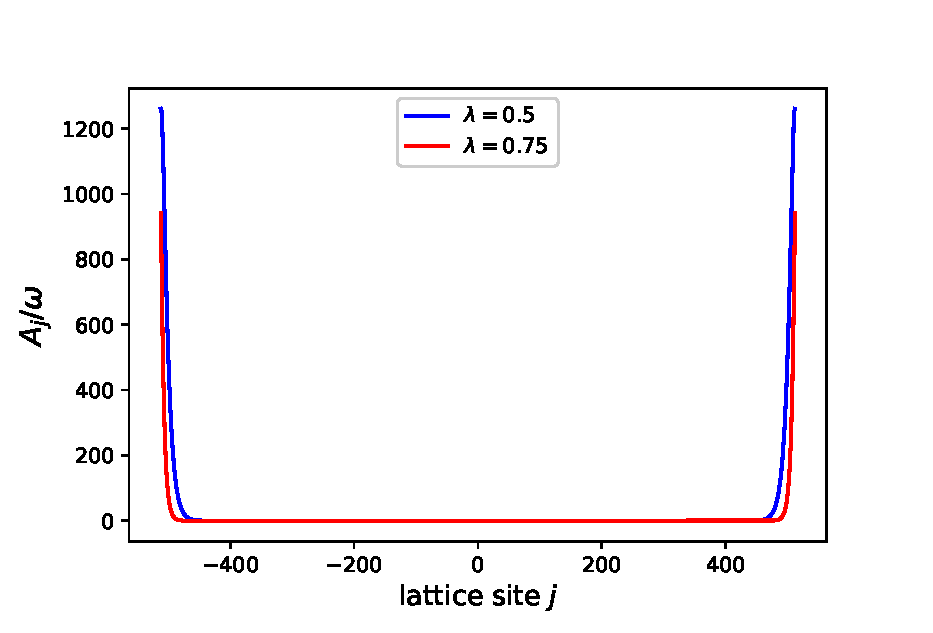
\includegraphics[scale=0.5]{pics/driving_field_amplitude.eps}
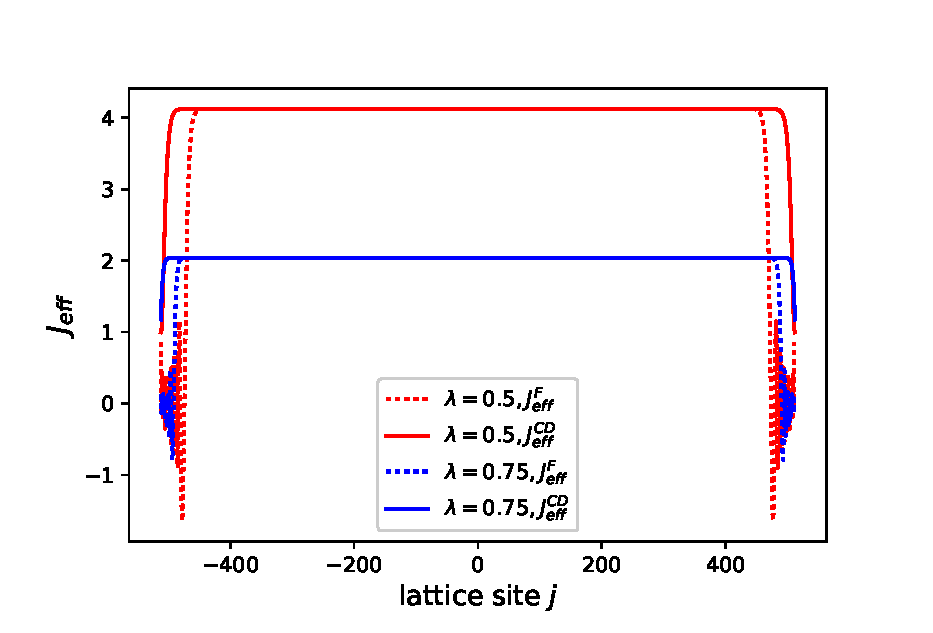
\includegraphics[scale=0.5]{pics/j_eff_f.eps}
\caption{a)   Driving field amplitude $A_j$ b)  Comparison of effective hopping strength from floquet and CD driving }
\end{center}
\end{figure}

\section{Eckart potential}

\subsection{Inserting potential}
$V(\lambda,j) =\dfrac{ \lambda(t)}{\cosh^2 j/ \xi}$ where $\xi$ is the localization length.


\begin{figure}[!ht]
\begin{center}
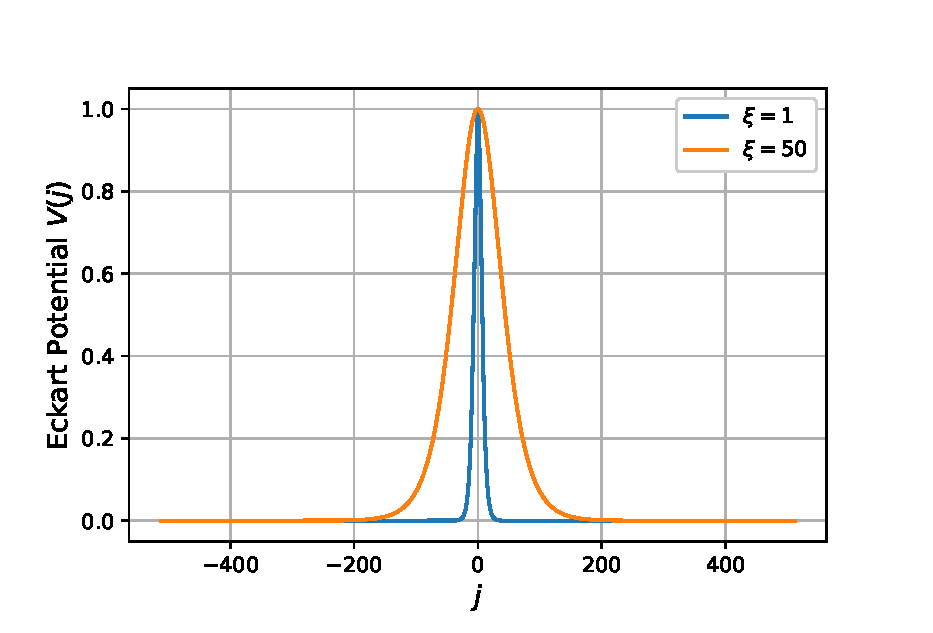
\includegraphics[scale=0.68]{pics/eckart_potn.eps}
\caption{Eckart potential with $\lambda=1$ }
\end{center}
\end{figure}

\begin{figure}[!ht]
\begin{center}
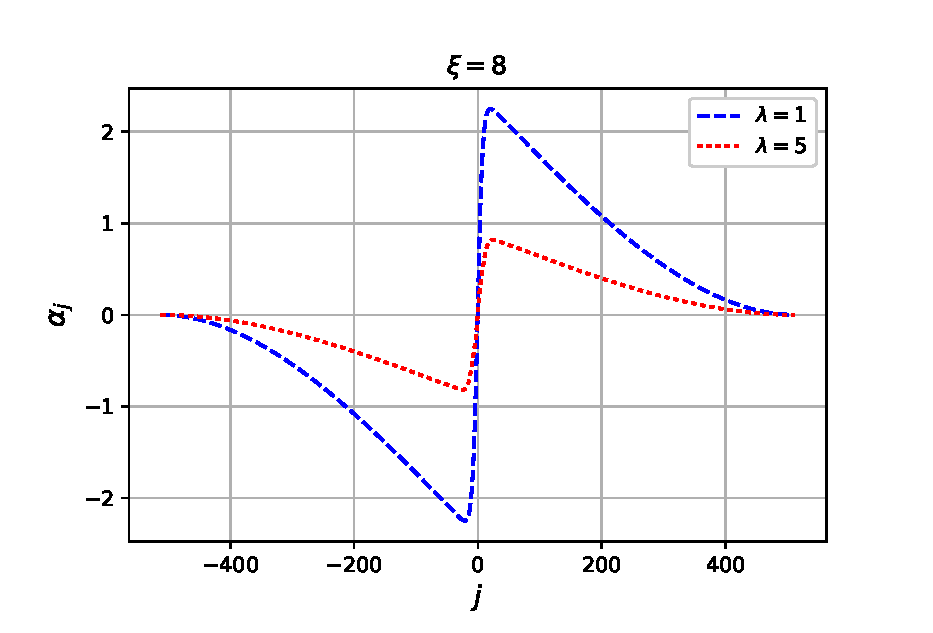
\includegraphics[scale=0.5]{pics/alpha_j_eckart_potn_loc.eps}
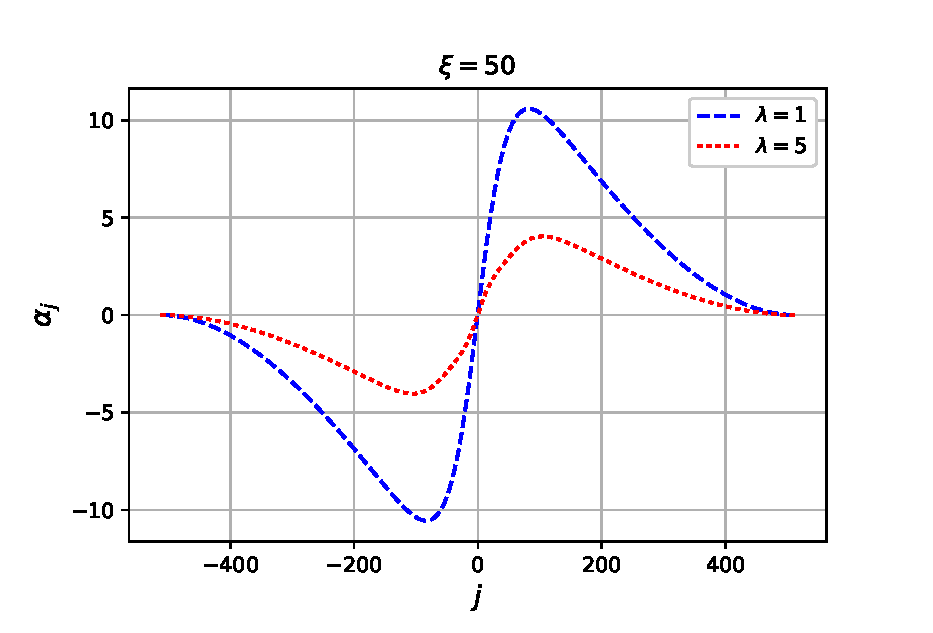
\includegraphics[scale=0.5]{pics/alpha_j_eckart_potn_nonloc.eps}
\caption{ $\alpha_j$ for Eckart potential  with vanishing boundary condition  with a) $\xi=8$ b) $\xi=50$}
\end{center}
\end{figure}


\begin{figure}[!ht]
\begin{center}
\includegraphics[scale=0.5]{pics/j_eff_cd_eckart_potn.eps}
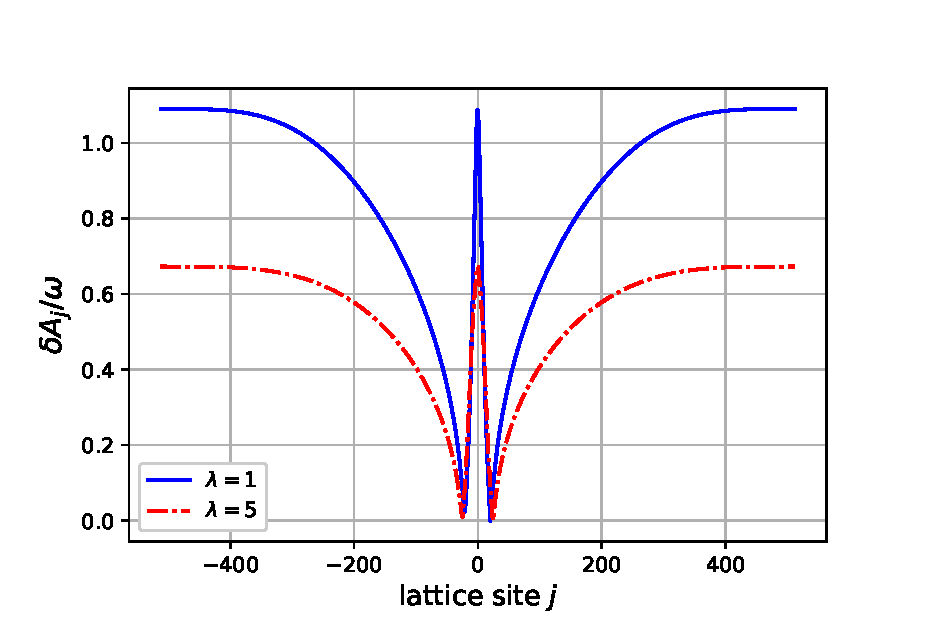
\includegraphics[scale=0.5]{pics/driving_field_amplitude_diff_eckart_potn.eps}
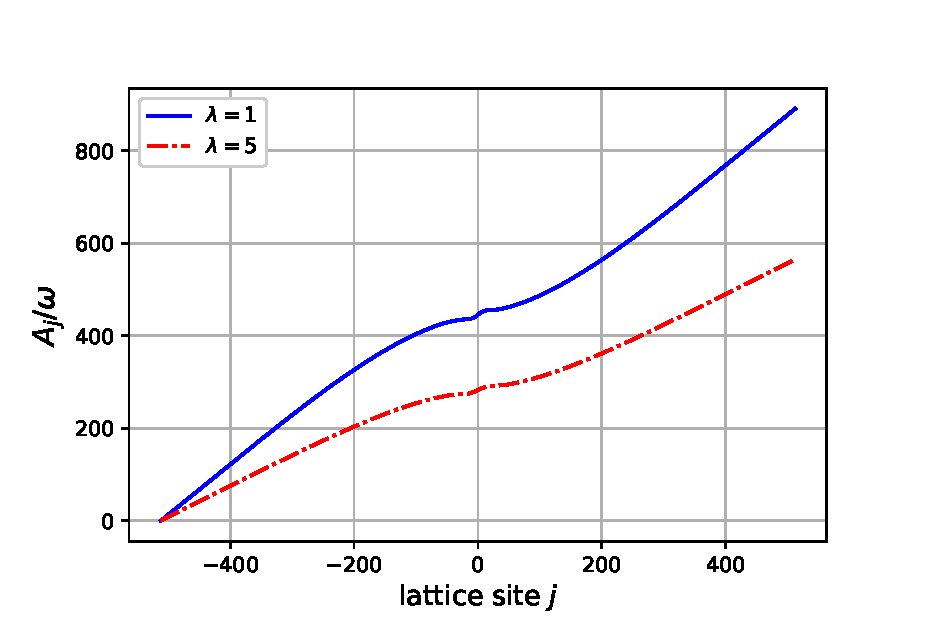
\includegraphics[scale=0.5]{pics/driving_field_amplitude_eckart_potn.eps}
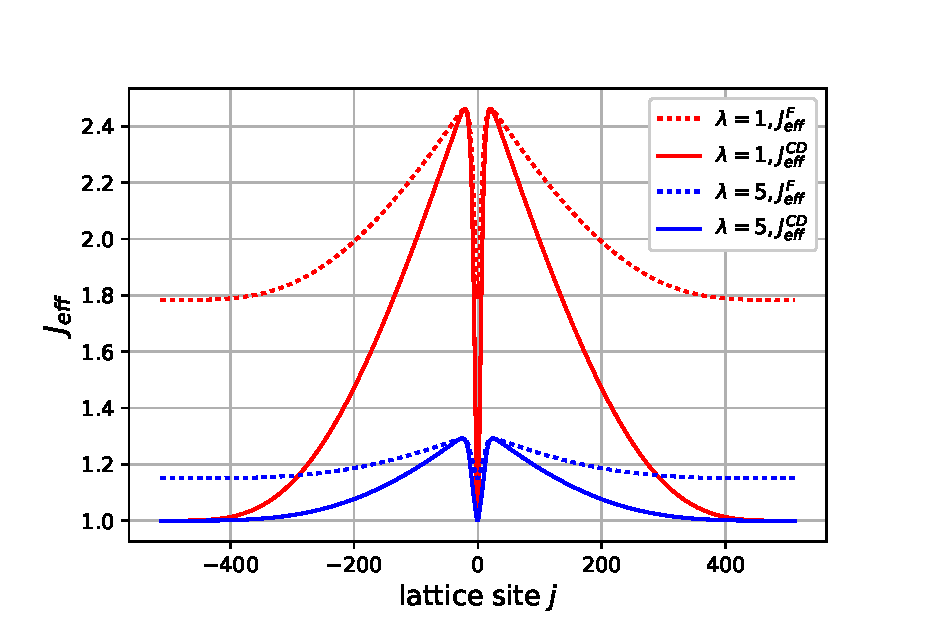
\includegraphics[scale=0.5]{pics/j_eff_comp_eckart_potn.eps}
\caption{ a) Effective hopping strength b) $(A_{j+1}-A_{j})/\omega$ c)Driving field's amplitude $A_{j}/\omega$ d) Comparison of effective hopping strength from floquet and CD driving }
\end{center}
\end{figure}

\subsection{Moving potential}
$V(\lambda,j) =\dfrac{V_0}{\cosh^2 [(j-\lambda)/ \xi]}$ where $\xi$ is the localization length.
We will use $V_0=2J$. And  $\partial_{\lambda}V=\dfrac{2V_0 \sinh [(j-\lambda)/ \xi]}{ \xi \cosh^3 [(j-\lambda)/ \xi]}=\dfrac{2V_0 \tanh [(j-\lambda)/ \xi]}{ \xi \cosh^2 [(j-\lambda)/ \xi]} $.

I still don't know why my numerical simulation is not consistent with Dries's calculation.

\appendix 
\section{Magnus expansion}
For a Hamiltonian which is periodic in time, it's unitary operator over a full driving cycle is given by:
\begin{equation}
U(T+ t_0, t_0)= \mathcal{T}_t\exp(- \dfrac{i}{\hbar} \int_{t_0}^T dt H(t))= \exp(- \dfrac{i}{\hbar}  H_F[t_0]T)
\end{equation}
$ H_F[t_0]= \sum_n H_F^{(n)}[t_0] $ 
where 
\begin{align*}
H_F^{(0)}= \dfrac{1}{T} \int_{t_0}^{T+t_0} H(t) dt \\
H_F^{(1)}= \dfrac{1}{2! T i \hbar} \int_{t_0}^{T+t_0}  dt_1\int_{t_0}^{t_1} dt_2  [H(t_1), H(t_2)] 
\end{align*}

Hence, 
\begin{align*}
|\psi (T) \rangle &= U |\psi (0) \rangle \\
&= \exp(- \dfrac{i}{\hbar}  H_F T)|\psi (0) \rangle \\
&= \lim_{\omega \rightarrow \infty}\exp(- \dfrac{i}{\hbar}  H_F^{(0)}T)|\psi (0) \rangle
\end{align*}


\section{Numerics of a single body problem}

Consider the Hamiltonian operator $\mathbf{H}$ on lattice 
\begin{equation}
\mathbf{H}= \sum_n V_n |n \rangle \langle n| + \sum_n (u_{n,n+1}|n \rangle \langle n+ 1|  + u_{n,n+1}^*|n +1 \rangle \langle n|)
\end{equation}
In units of $\hbar=1$, time-evolution is given by 
\begin{equation}
\mathbf{H} | \Psi \rangle= i\dfrac{d}{dt} | \Psi \rangle
\label{shrod eqn}
\end{equation}
We choose $| \Psi \rangle= \sum_n \psi_n | n \rangle$, where $\psi_n$ is the probability amplitude for the quantum particle on $n$-th lattice site. Hence, we find time-evolution of $\psi_n$ is given by:
\begin{equation}
i\frac{d\psi_n}{dt} =   u_{n,n+1}\psi_{n+1} + u_{n-1,n}^* \psi_{n-1} + V_n \psi_n 
\end{equation}
With this, we have converted the problem of solving SE into a problem of solving an ODE.

For us, $u_{j, j+1}= \exp\left(i \sin(\omega t) \dfrac{A_{j+1}- A_j}{\omega}\right)$ as we are interested in studying the dynamics of this Hamiltonian:
\begin{align*}
H&= J\sum_{j=0}^{L-1}   ( u^{j, j+1} c_{j+1}^{\dagger} c_j + \mbox{h.c}) 
\end{align*}
where periodic boundary condition is assumed. Let's suppose $A_j= j$ where $j$ goes from $0$ to $L-2$ and $A_{j=L-1}= 0$ so that $A_{j+1}- A_j=1$ for all values of $j=\{0,L-1\}$ \footnote{We should be careful with the boundary terms. For $j={0,L-1}$, $A_1-A_0=1$. But $A_{L}-A_{L-1}=A_0- (L-1)=1-L$}. For a lattice-size of $L=51$, I did numerical simulation with initial condition as $| \psi (t=0) \rangle= \delta_{i, (L-1)/2}$.



\begin{equation*}
\begin{aligned}[c]
|\psi (t=T)_{num} \rangle &= U |\psi (0) \rangle \\
&= \exp(- \dfrac{i}{\hbar}  H T)|\psi (0) \rangle 
\end{aligned}
\qquad \qquad
\begin{aligned}[c]
|\psi_F (T) \rangle &= U_F |\psi (0) \rangle \\
&\simeq \exp(- \dfrac{i}{\hbar}  H_F^{(0)}T)|\psi (0) \rangle
\end{aligned}
\end{equation*}

where $H_F^{(0)}= \sum_{j=0}^{L-1} J_{j}^F (c_{j+1}^{\dagger} c_j + \mbox{h.c})$ with $J_{j}^F=J^F \mathcal{J}_0 \left(\dfrac{A_{j+1}- A_j}{\omega}\right)$

\begin{figure}[!ht]
\begin{center}
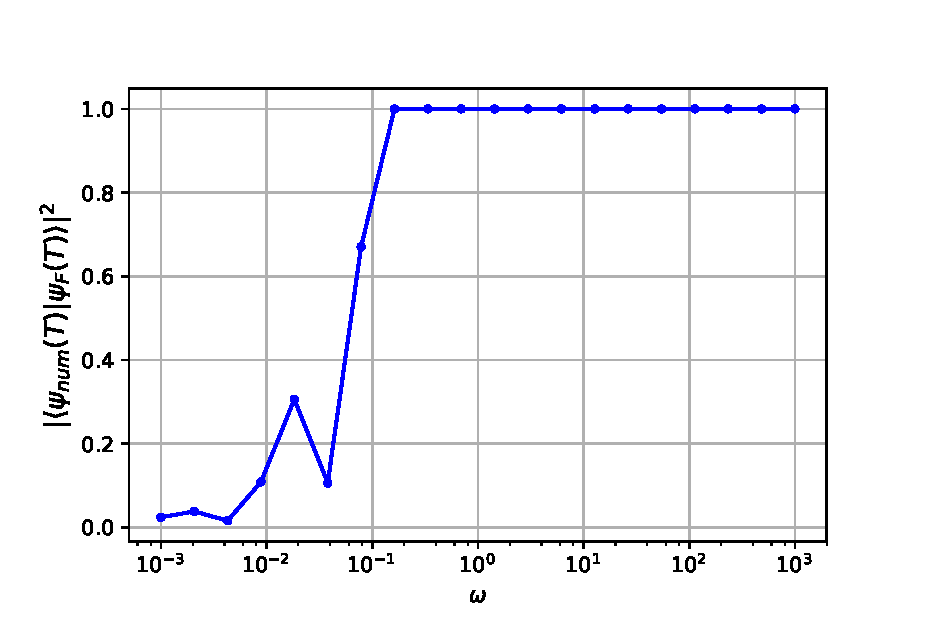
\includegraphics[scale=0.5]{pics/single_body_L51_floquet.eps} 
\caption{$\psi_{num}(T)$ is the wavefunction obtained after solving numerically and $\psi_F (T)$ is the wevfunction-obtained using zeroth term of Magnus expansion}
\end{center}
\end{figure}
\section{Bessel's function of first kind}
Integral representation of Bessel's function of first kind $\mathcal{J}_n (x)$ is given by:
\begin{equation}
\mathcal{J}_n (x)=  \frac{1}{2 \pi} \int_{-\pi}^\pi d\tau e^{i(n \tau - x \sin \tau)}= \frac{1}{T} \int_{-T/2}^{T/2} d\tau e^{i(n   \omega \tau - x \sin \omega \tau)}
\end{equation}
For $x \ll1$, $\mathcal{J}_0 (x)= 1- \frac{x^2}{2}$

\begin{figure}[!ht]
\begin{center}
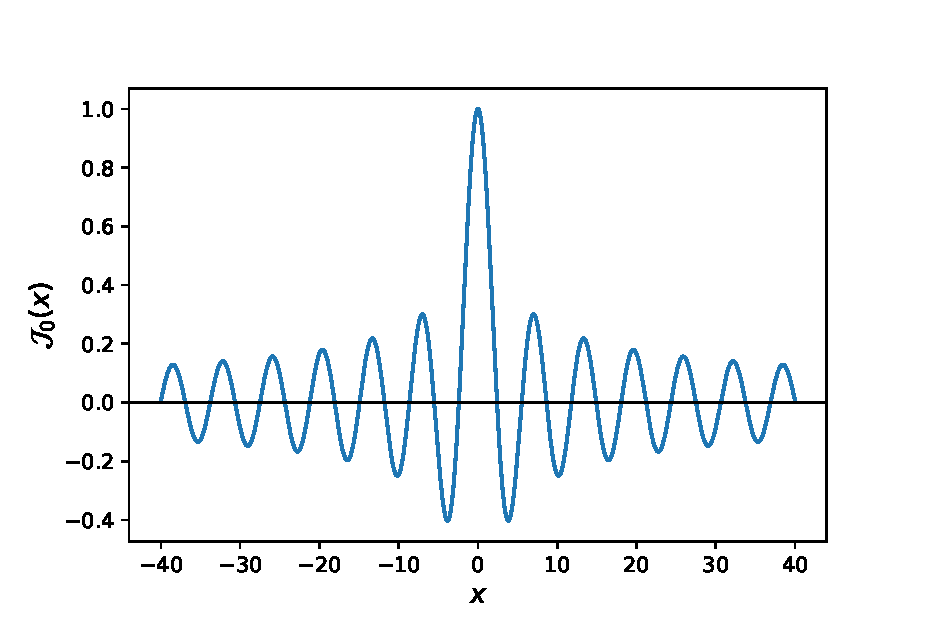
\includegraphics[scale=0.5]{pics/bessel_fun.eps} 
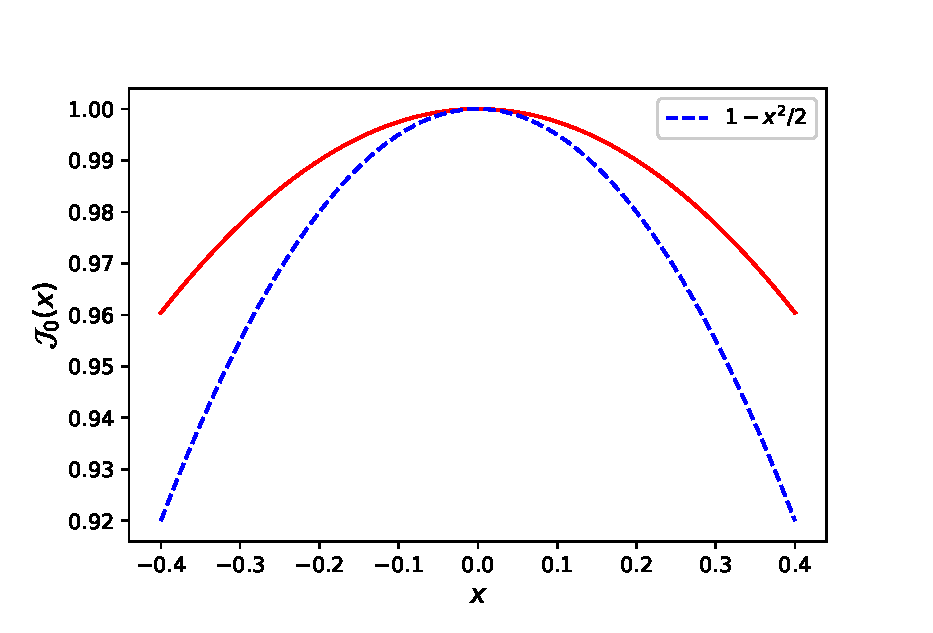
\includegraphics[scale=0.5]{pics/bessel_fun_zoom.eps} 
\caption{Bessel's function }
\end{center}
\end{figure}

%\subsection{Matrix representation}
\bibliography{ref} 

\bibliographystyle{unsrt}
%\bibliographystyle{plain}

\end{document}
